% https://www.zhihu.com/question/594688809/answer/2012912802805855581
\documentclass[tikz,border=5pt]{standalone}
\usetikzlibrary{arrows.meta}
\begin{document}
    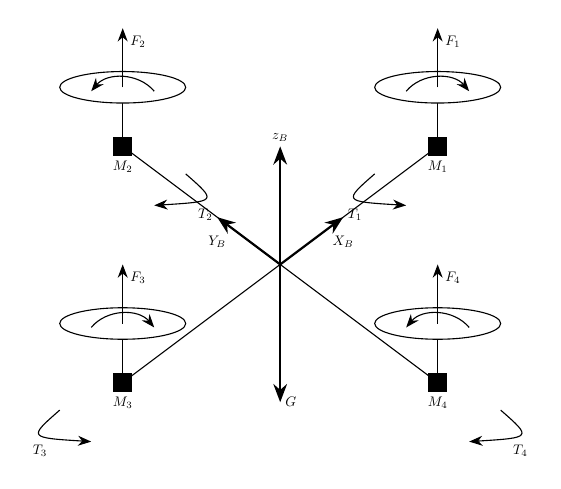
\begin{tikzpicture}[
        >=Stealth,
        myplane/.cd,
        base-x/.initial=1,
        axis-x/.initial=1,
        basedir/.is choice,
        basedir/left/.style={base-x=1},
        basedir/right/.style={base-x=-1},
        axisdir/.is choice,
        axisdir/left/.style={axis-x=1},
        axisdir/right/.style={axis-x=-1},
        basedir/.initial=left,
        axisdir/.initial=left,
        labelnum/.initial=,%
        /tikz/pics/myplane/.style={
            code={
                \draw (0,0) node[rectangle,fill=black,label={[scale=.5]below:$M_\pgfkeysvalueof{/tikz/myplane/labelnum}$}] {} -- ++(0,.75) coordinate (tmp);
                \begin{scope}[xscale=\pgfkeysvalueof{/tikz/myplane/base-x}]
                    \draw[->] (0,0) +(.8,-.35) .. controls +(.4,-.35) .. +(.4,-.75) node[midway,below=2pt,scale=.5] { $T_\pgfkeysvalueof{/tikz/myplane/labelnum}$};
                \end{scope}
                \draw[fill=white] (tmp) ellipse [x radius=.8, y radius=0.2];
                \draw[->] (tmp) -- ++(0,.75) node[below right=1pt,scale=.5] {$F_\pgfkeysvalueof{/tikz/myplane/labelnum}$};
                \begin{scope}[xscale=\pgfkeysvalueof{/tikz/myplane/axis-x}]
                    \draw[->] (tmp) ++(.4,-.05) to[bend right=50] ++(-.8,0);
                \end{scope}
            }
        }
    ]

% \pic {myplane};

% \pic[myplane/.cd,basedir=left,axisdir=right] at (3,0) {myplane};

% \pic[myplane/.cd,basedir=right,labelnum=t] at (6,0) {myplane};

\coordinate (O) at (0,0);
\draw (O) -- +(2,1.5) coordinate (A)
    (O) -- +(-2,1.5) coordinate (B)
    (O) -- +(-2,-1.5) coordinate (C)
    (O) -- +(2,-1.5) coordinate (D);

\draw[thick,->] (O) -- +(0,1.5) node[above,scale=.5] {$z_B$};
\draw[thick,->] (O) -- +(0,-1.75) node[right,scale=.5] {$G$};
\draw[thick,->] (O) -- +(-.8,.6) node[below=5pt,scale=.5] {$Y_B$};
\draw[thick,->] (O) -- +(.8,.6) node[below=5pt,scale=.5] {$X_B$};

\pic[myplane/.cd,labelnum=1,axisdir=right,basedir=right] at (A) {myplane};

\pic[myplane/.cd,labelnum=2,] at (B) {myplane};

\pic[myplane/.cd,labelnum=3,axisdir=right,basedir=right] at (C) {myplane};

\pic[myplane/.cd,labelnum=4,] at (D) {myplane};

\end{tikzpicture}

\end{document}